\subsubsection{Moving average filter} \label{sec:mavg_test}
Moving average filteret testes for at undersøge, hvorvidt de opstillede krav overholdes, samt undersøge om designet er korrekt implementeret. Måden, hvorpå dette testes er ved anvendelse af data fra pilotforsøget, da dette giver kontrolleret testforhold. 
MATLAB benyttes til at sende en given måling til mikrokontrolleren, hvorpå det digitale filter er implementeret. Mikrokontrolleren returnerer løbende den filtrerede værdi, der visualiseres i MATLAB. Ud fra dette ses om filteret udglatter signalet som forventet. 
Resultatet af denne test fremgår af \autoref{fig:mavg_test}. 

\begin{figure}[H]
	\centering
	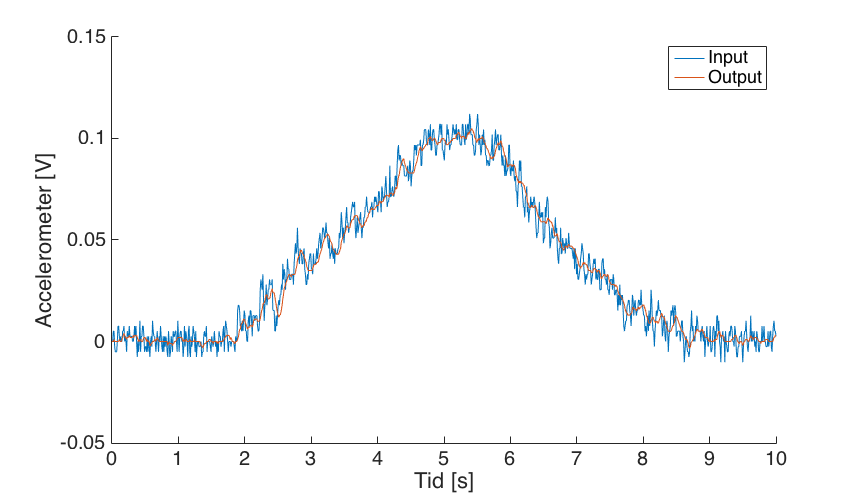
\includegraphics[width=1\textwidth]{figures/accelerometer_filter}
	\caption{Den blå graf illustrerer et opsamlet ufiltreret signal fra accelerometer og den røde graf illustrerer et opsamlet filtreret signal fra accelerometer, visualiseret i MATLAB}
	\label{fig:mavg_test}
\end{figure}

\noindent
%Da filteret kræver 10 samples for at retunere den første værdi testes det, hvorvidt dette stemmer overens med den forventede forsinkelse på $100~ms$. 
Der foretages yderligere en test med fremgangsmåde som i den forrige. Hertil er et anvendes et square-wave signal genereret i MATLAB. Dette signal sendes igen ind i mikrokontrolleren, hvor filter er implementeret, og de filtreret data returneres. En visualisering af denne test ses af \autoref{fig:forsinkelse}

\begin{figure}[H]
	\centering
	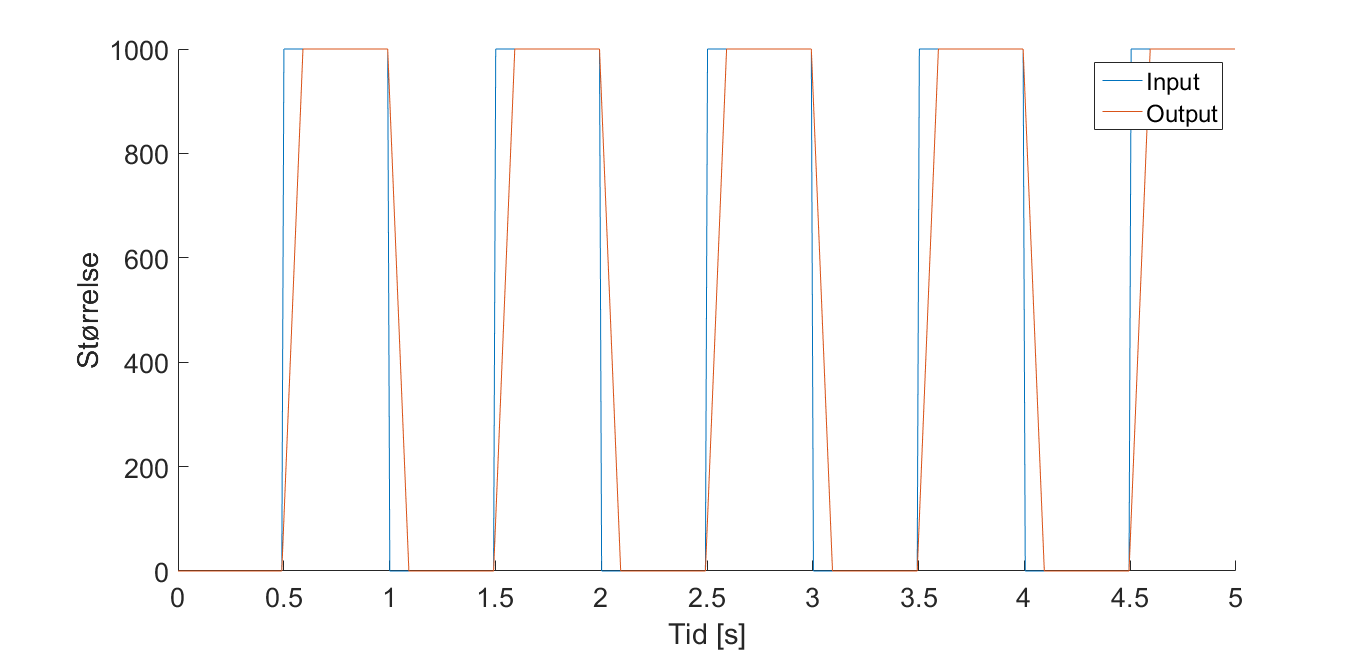
\includegraphics[width=1\textwidth]{figures/forsinkelse}
	\caption{Den blå graf illustrerer et genereret signal, og den røde graf illustrerer det opsamlet filtreret signal.}
	\label{fig:forsinkelse}
\end{figure}

\noindent
Resultat af denne test viser at moving average filteret udglatter signalet. Hertil ses det at der er en stigning i det genreret signal før det filtreret signal når den samme størrelse. I mellem dette går der $0,09~s$. Dette er passende til mængden af samples som filterets gennemsnit er udregnet ud fra ved en samplingsfrekvens på $100~Hz$. 
Dette er lavere end forventet, da der udfra $10~samples$ forventes at tage $0,1~s$. Hvortil filteret accepteres .  

Yderligere foretages en test af forsinkelsen. Testen er udført på samme måde som forklaret i \autoref{sec:lavpas_test}. Resultatet fra testen er en forsinkelse på $320~\mu s$ for data at passere filteret. Dette betragtes som værende ikke af signifikant betydning.    
Ud fra ovenstående resultater vurderes det, at det filterede signal opfylder kravene for \autoref{sec:mavg_krav}. 


\vspace{3mm}
\textbf{Opsummering af krav:}
\begin{itemize}
\item[\text{\sffamily \checkmark}] Skal muliggøre en repræsentation af spændinger 
\item[\text{\sffamily \checkmark}] Skal have en filterlængde på $10$ samples
\item[\text{\sffamily \checkmark}] Skal maksimal tage $100~ms$ for at opnå samme værdi som det oprindelige signal ved en konstant amplitude.
\end{itemize}